
\chapter{Implementation}

This chapter describes the implementation of the features that were added to \ac{AnSiAn}. We roughly describe the theoretical background, the design choices made and the actual implementation in Java. Additionally we extensively describe the challenges we faced during the implementation. 

\section{Feature 1: Transmission Chain}


\begin{figure}
	\centering
	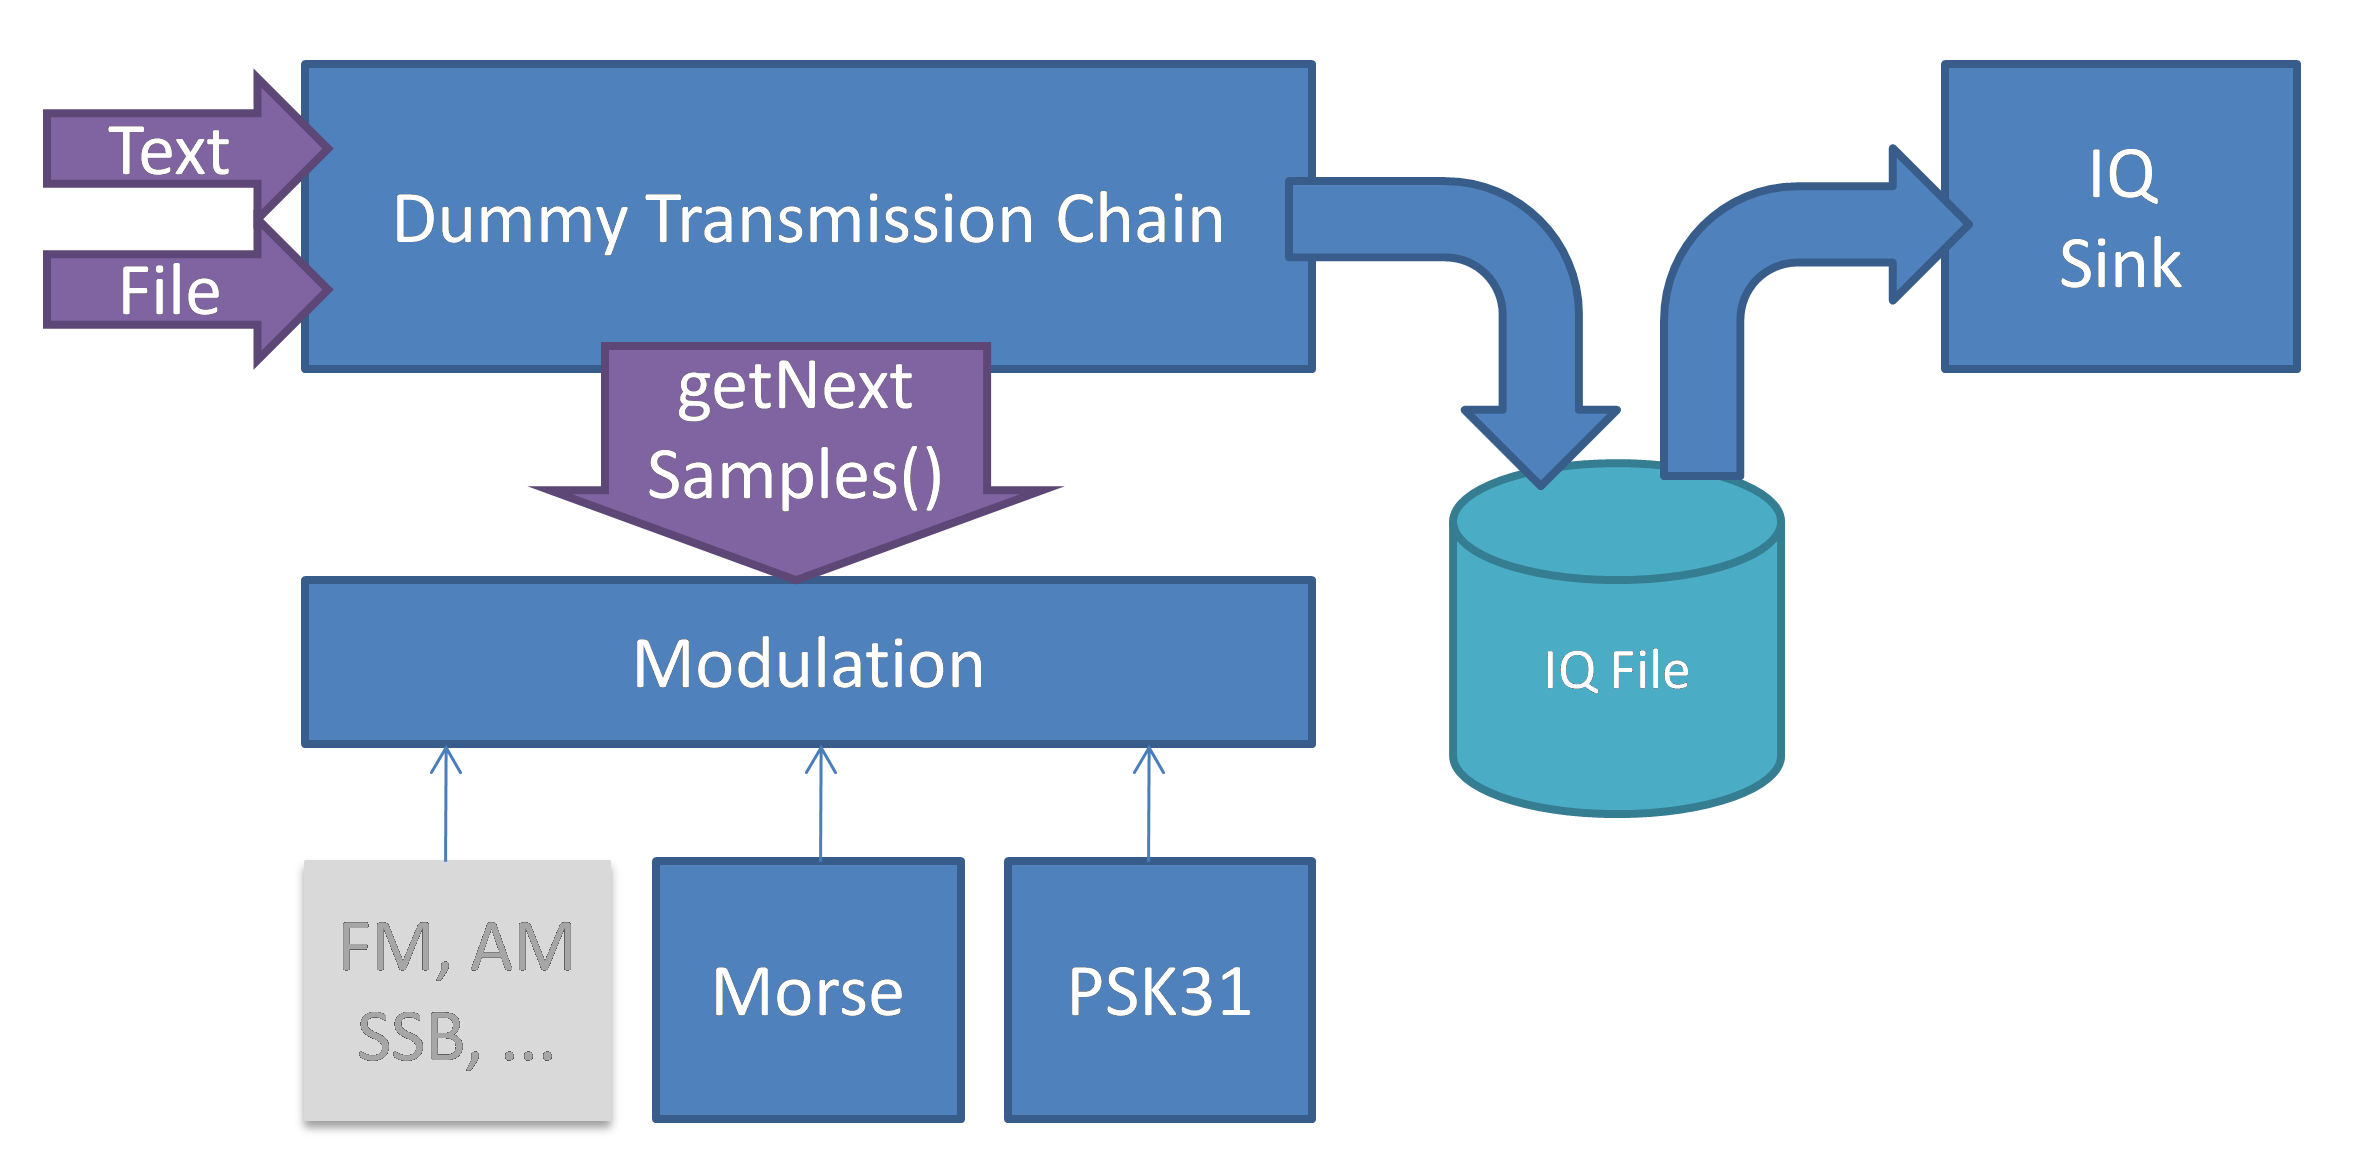
\includegraphics[width=1\linewidth]{gfx/TX_chain_step2.png}
	\caption{Transmission in current version of AnSiAn \cite{Mantz2016}}
	\label{fig:tx_chain_old2}
\end{figure}


Figure~\ref{fig:tx_chain_old2} illustrates the implementation of the transmission before our project started. We roughly analyze how this has been implemented to find out the main problems of the implementation. The DummyTransmissionChain is the entry point of a transmission. It is called when the user initializes a transmission. The different modulations (currently PSK31 and Morse) are implemented as a subclass of Modulation. The DummyTransmissionChain repeatedly calls getNextSamples() to get a SamplePacket of the selected Modulation until it returns null. The SamplePacket is basically a complex array (i.e. 2 float arrays containing in-phase and quadrature components). The DummyTransmissionChain then serializes this to a signed 8 bit integer IQ File, i.e. converts floats to bytes and interleaves I and Q samples. Once the Modulation is done, the IQSink is launched which reads the file and passes it to the HackRF driver using the BlockingQueue of byte buffers provided by the HackRF driver. 

\pagebreak
With this implementation we see the following problems: 
\begin{itemize}
	\item The modulation is entirely done before the transmission is start-ed. This is not only very inconvenient for the user since he has to wait for a long time before the transmission starts, but it also is not suitable for the features we want to implement where we require continuous transmission of recorded audio. We want to implement this in a way where the modulation is done simultaneously to the transmission. Mantz and Engelhardt \cite{Mantz2016} already described a concept to use BlockingQueues, i.e. we queue up N packets and then block until a packet has been removed from the queue. This helps to have enough samples ready, but not using too much memory, which is a rare resource on smartphones. 
	\item Writing to a file introduces additional overhead. This was done to save memory, but is not required if we can do the modulation just-in-time. 
	\item The format of the file is currently limited to interleaved I/Q 8-bit signed integers. It would be nice to support other formats as well. 
	\item Aborting a transmission currently takes a few seconds due to the implementation of the IQ Sink. 
	\item Currently only the sampling rate of 1MHz is supported. This is not a real problem at the moment, but it might be nice in the future to be able to use different input and output sample rates for the transmission chain.
\end{itemize}

\label{sec:impl:feature1}
\subsection{Structural Changes}
\begin{figure}
	\centering
	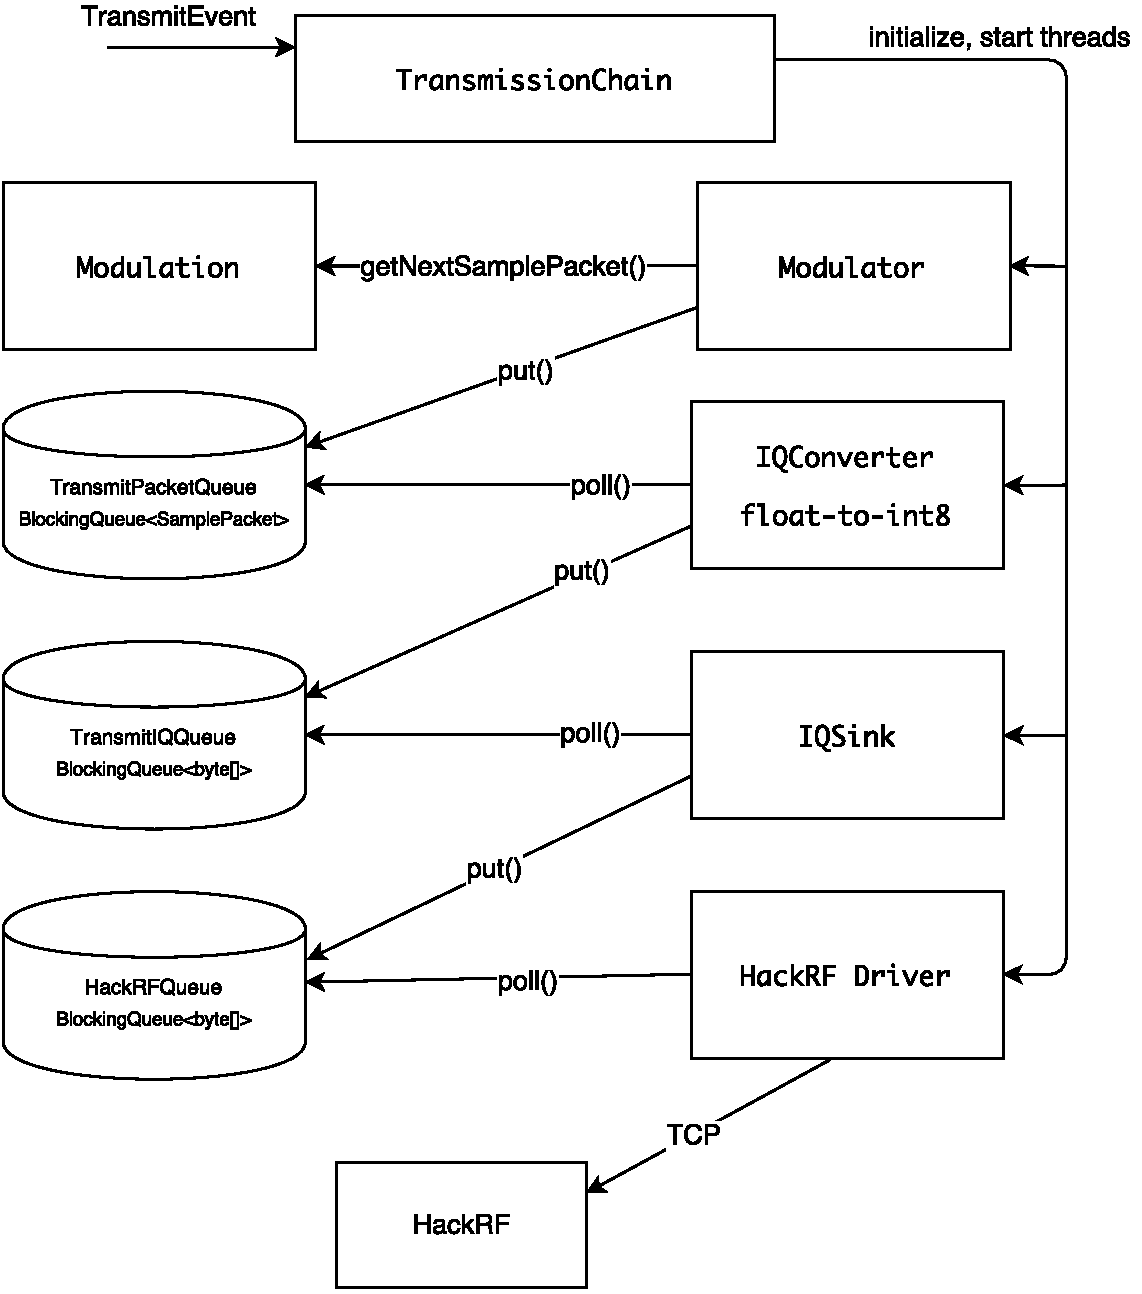
\includegraphics[width=0.8\linewidth]{gfx/feature1_design.pdf}
	\caption{Implementation of the Transmission Chain}
	\label{fig:impl:transmissionchain}
\end{figure}
To solve the problems detected with the old implementation we needed to adjust the architecture of the transmission chain. The current transmission chain is outlined in Figure~\ref{fig:impl:transmissionchain}. We briefly describe the responsibilities of each component: 

\begin{itemize}
	\item \textbf{TransmissionChain}: Responsible to launch the transmission chain. It listens to TransmitEvents that were sent by the UI. It is the only object that is created on app startup and is kept in memory for the entire time - all other parts of the transmission chain are started for a single transmission and die afterwards. Ideally this class is the only one that contains Android specific / dependent code. 
	\item \textbf{Modulator}: The Modulator continuously gets SamplePackets from the correct Modulation and pushes them to the TransmitPacketQueue. 
	\item \textbf{IQConverter}: Converts the SamplePackets (float) from the TransmitPacketQueue to the required data format (For HackRF: 8bit IQ samples). The data is filled into byte buffers that are then enqueued into the TransmitIQQueue. 
	\item \textbf{IQSink}: Configures the HackRF Driver. Then continuously takes the buffers from the TransmitIQQueue and passes them to the driver specific Queue. 
\end{itemize}

We decided not to implement an interpolator at first, which would have enabled to use different sampling rates for modulating than for the actual transmission. We did this because currently we are using 1 MHz everywhere. If we require different sampling rates later this can be easily added. 

\subsection{Implementation}

After we described the structural changes and required classes in the last section, we now point out a few specific implementation choices that were made during the development: 
Since we need to run the components concurrently and we do not want to do a lot of work on the main thread, we need to make use of multiple threads. When a transmission is initialized the TransmissionChain object quickly creates a object of each component and then runs each in a separate thread. \\
We already described the concept of Blocking Queues. This highly simplifies the implementation of the chain, since we do not need to take of the communication and memory management. The threads just do their work and enqueue the results in the next queue and the rest is controlled by the queue limits. We only need to decide how long the queues are. The byte buffers have a size of 16 KiB (as defined by the HackRF driver), while the SamplePackets can have arbitrary size (usually a lot bigger). Therefore we currently choose 5 as the maximum size of the TransmitPacketQueue and 200 for the TransmitIQQueue.  
	
It is important to keep memory management in mind. If every component just keeps allocating new memory the application will run out of memory or the Java Garbage Collector will be to busy and drastically slow down the application. Therefore we use the buffer pool for the byte buffers of the HackRF driver. This again uses BlockingQueues, which makes sure that only a fixed number of buffers are used throughout the application.  
	
All components need to be interruptible. This needs to be implemented by the class itself. The TransmissionChain can only call the .interupt method of the thread, but the thread itself needs to take care that this interupt is received and correctly handled. 
	
The implementation of the IQConverter was more challenging than expected. The main challenge is that the size of the SamplePackets can be different than and even not divisible by the buffer size required by the IQSink. We decided to memorize the last samples of the SamplePacket until the next SamplePacket is processed. However we can not know if a SamplePacket is the last one. Therefore we implemented that that if no SamplePacket arrives for a specified time (here 1000 ms), we fill the rest of the buffer with zeros and transmit it. 


\subsubsection{Debugging and Testing}
Since all software contains bugs, we needed to find a way to find a way to debug and test our implementation in a convenient and fast way. We developed unit tests for the IQConverter, since it contains logic that can be easily tested by a unit test. 

To test the other components we wanted to monitor the bytes that are actually passed to the HackRF driver. To do so we implemented a FileIQSink, that can be launched instead of the normal IQSink. This FileIQSink writes the samples to a file. Then we transfered this file to a computer and analyzed them with Matlab, Audacity and a Hex editor. 
After we successfully fixed a lot of smaller bugs in our implementation, we integrated it into the current application and performed manual regression tests of the already implemented transmission features. We tested our implementation with the 3 currently implemented transmission modes: 
\begin{itemize}
	\item Morse Code Modulation
	\item PSK31 with USB Modulation
	\item Directly transmitting a IQ File 
\end{itemize}

All three transmission modes are now working without any problems and do no longer require long calculations before the transmission. 



\section{Feature 2: RDS Transmission}
\label{sec:impl:feature2}
The second feature implements the synthesis of \ac{RDS} signals. \ac{RDS} has been standardized by the RDS Forum \cite{RDS1999}. It is a good example for a non-trivial protocol that is very widely used. We wanted to demonstrate that these signals can be synthesized on a smartphone, such that a commodity kitchen or car radio is able to decode them. 

One of the main features of RDS is the transmission of the station information (station name, audio information, station location and other meta data about the transmission). Most radios only display the station name. This is why we are also concentrating on this feature. 

The RDS signals are transmitted together with the audio signal using frequency modulation. By implementing RDS in AnSiAn, we enables the user to broadcast his own radio signals with a station name specified by the user. 

\subsection{User Interface}
\begin{figure}
	\centering
	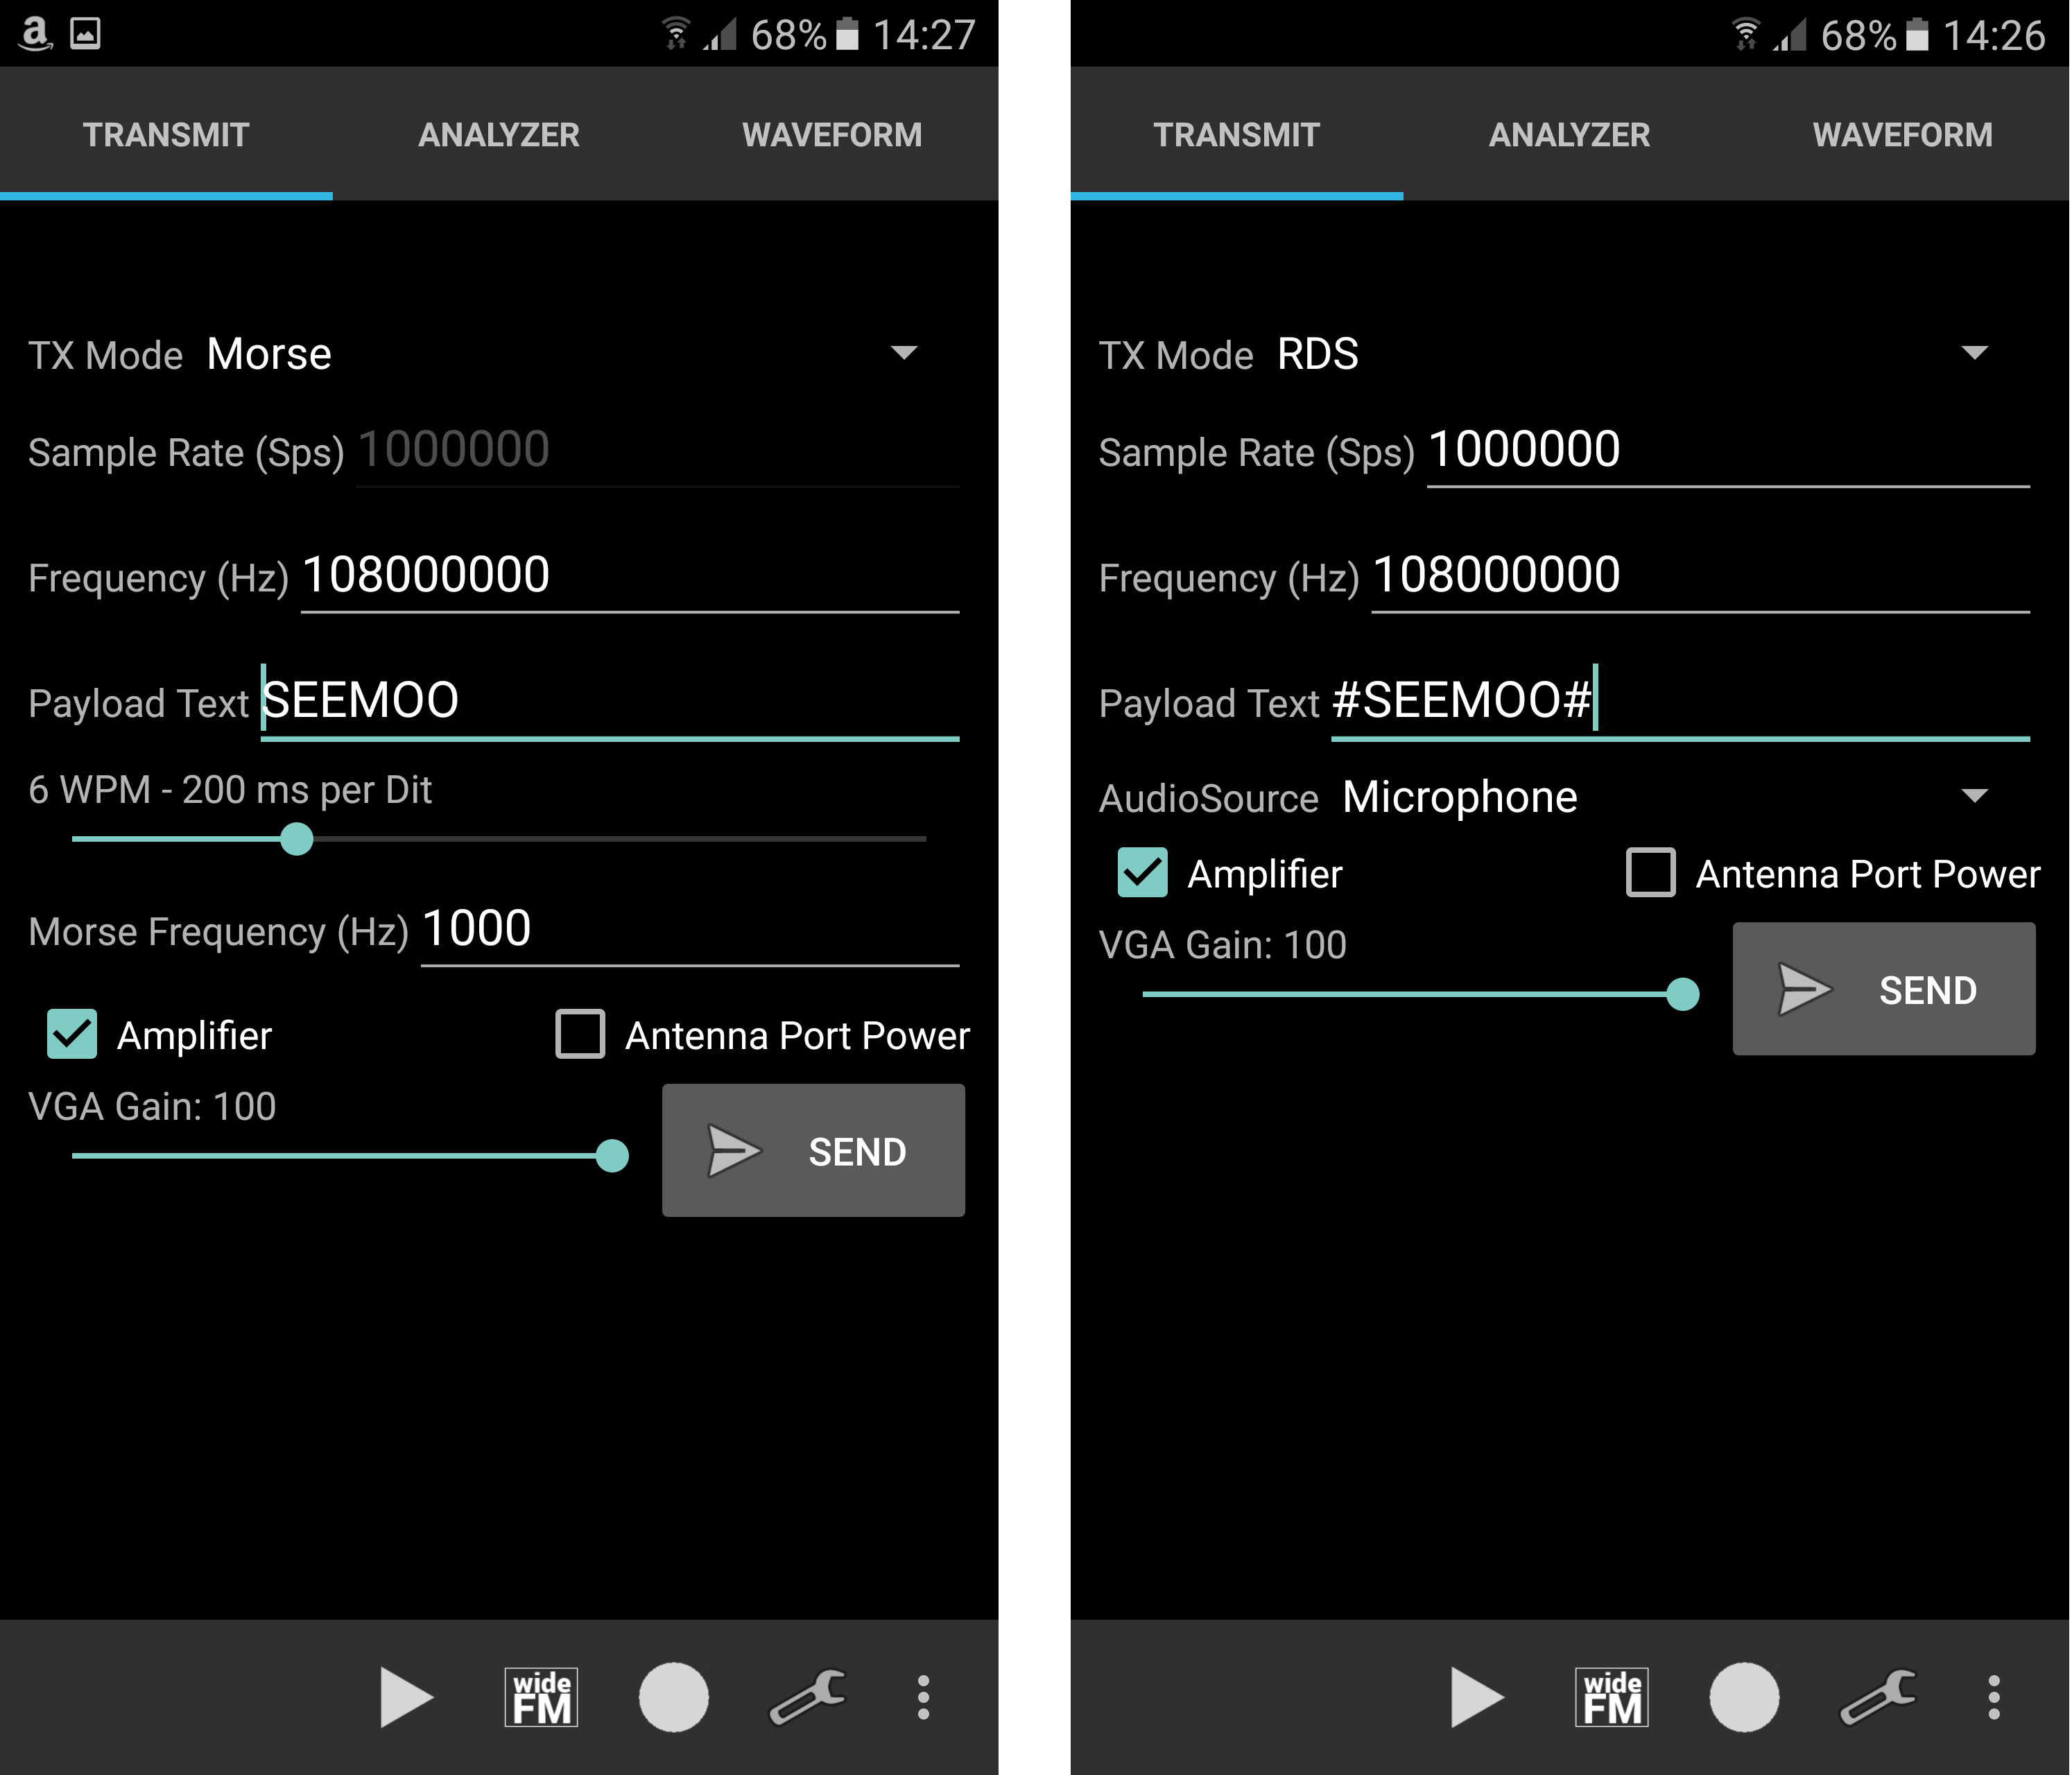
\includegraphics[width=1.0\linewidth]{gfx/screenshot_rds.png}
	\caption{AnSiAn Transmission Tab: Morse (old, left) and RDS (new, right)}
	\label{fig:impl:screenshotrds}
\end{figure}


Figure~\ref{fig:impl:screenshotrds} shows a screenshot of the extended transmission tab of AnSiAn. For reference we printed the already existing Morse transmission screen on the left. On the right you can see the newly added screen which enables the user to transmit RDS signals. The user can enter his own station name (at most 8 characters) and select an audio source (currently we are supporting the integrated microphone and a audio file source). The other settings are the same as for the other transmission modes. 


\subsection{Implementation}
To transmit a radio signal including RDS, we need to do the following steps (c.f. \cite{RDS1999}):

\begin{enumerate}
	\item Generate a bit string according to RDS specification (4 groups, each 64 bit)
	\item Calculate 10 bit check words for every 16-bit block (resulting in 4 groups, each 104 bits)
	\item Calculate differential encoding of the bit string
	\item Manchester encode the bit string
	\item Apply a low-pass filter to the signal to cut off frequencies higher than 2800 Hz
	\item Upconvert the generated signal to 57 kHz
	\item Add a sinusoidal pilot tone at 19 kHz
	\item Add the base band audio signal (only containing low frequencies). Most audio signals are sampled at 44100 Hz. So we need to resample these signals to match our sampling rate of 1MHz. 
	\item Calculate the frequency modulation on the signal with a frequency deviation of 75000 kHz 	
\end{enumerate}

\begin{figure}
	\centering
	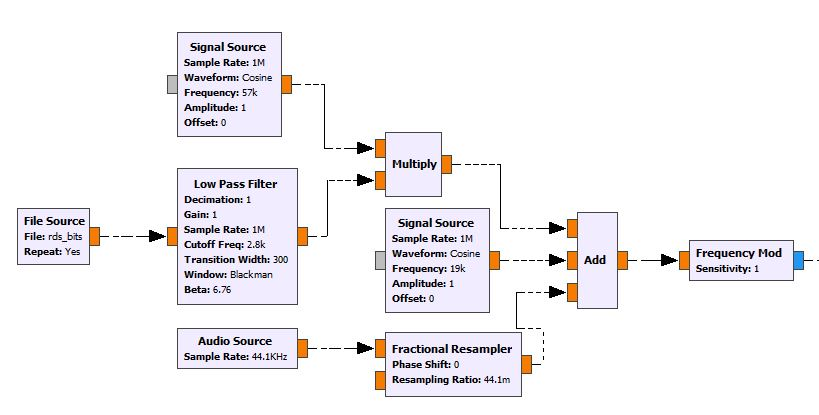
\includegraphics[width=1.3\linewidth]{gfx/rds_gnu.jpg}
	\caption{GNU Radio flow graph of RDS signal generation}
	\label{fig:impl:rdsgnu}
\end{figure}

The steps after step 4 are illustrated in the GNU radio flow graph in Figure~\ref{fig:impl:rdsgnu}. Since most of these steps are pretty straight forward we only explain the more complex ones in detail here. For the bit string generation and check word calculation refer to the documentation of the RDS decoding functionality implemented in AnSiAn (The documentation of that can be found in \cite{Mantz2016} in Section 4.2.3). 

\subsubsection{Low-Pass Filtering}

AnSiAn already contains a implementation of a Blackman Low-Pass filter. The signature of the low pass filter function is shown in Listing~\ref{lst:javacreatelowpass}

\begin{lstlisting}[label=lst:javacreatelowpass, caption=AnSiAn Blackman Low-Pass Filter, language=java]
// create a filter 
public static FirFilter createLowPass(int decimation, float gain, 
   float sampling_freq, // Hz
   float cutoff_freq, // Hz BEGINNING of transition band
   float transition_width, // Hz width of transition band
   float attenuation_dB) // attenuation dB
   
// filter 
public int filterReal(SamplePacket in, SamplePacket out, int offset, int length)    

\end{lstlisting}
However the choice of its parameter highly influences the performance of the filter. A bad parameter choice either leads to a badly filtered signal or to a very long filtering time. Since we are very constrained in terms of computing power on the Android platform, we want to choose the parameter such that the filter is just good enough but still very fast. 
We found that the best parameter choice for us was cutoff\_freq=2800Hz, transition\_width=300Hz and attenuation\_dB=3dB. \\
The parameters decimation=1, gain=1 and sampling\_freq=1000000 are fixed for us. 

\subsubsection{Frequency Modulation}

For implementing frequency modulation, we looked the implementation in the Octave communications package. Listing~\ref{lst:octave_fmmod} shows how Octave implements fmmod. 
\lstset{numbers=left}
\lstset{stepnumber=1}
\begin{lstlisting}[label=lst:octave_fmmod, caption=Octave implementation of Frequency modulation \cite{octavefmmod}, language=octave,]
function s = fmmod (m, fc, fs, freqdev)
   l = length (m);
   t = 0:1./fs:(l-1)./fs;
   int_m = cumsum (m)./fs;
   s = cos (2*pi.*fc.*t + 2*pi.*freqdev.*int_m);
endfunction
\end{lstlisting}

It implements the following function 

\begin{equation}
 s(t) = cos\left(2\cdot \pi \cdot f_c \cdot t + 2\cdot \pi\cdot f_\Delta \int_{0}^{t}m(t')dt'\right)
\end{equation}

However this modulates the signal in the pass band, but we require it in the base band and the up conversion is done later by the HackRF. Therefore we can either set $f_c=0$ or use 

\begin{equation}
s(t) = cos\left(2\cdot \pi \cdot f_\Delta  \cdot \int_{0}^{t}m(t')dt'\right)
\end{equation}


The implementation in Java is straight forward and shown in Listing~\ref{lst:javafmmod}.
\begin{lstlisting}[label=lst:javafmmod, caption=Java Implementation of fmmod, language=java,]
public static SamplePacket fmmod(float[] x, float fs, float freqdev ){
   SamplePacket packet = new SamplePacket(x.length);
   packet.setSize(x.length);
   float[] sum = cumsum(x);
   for(int i=0;i<sum.length;i++){
      sum[i] = sum[i]/fs;
   }
	
   float[] re = packet.getRe();
   float[] im = packet.getIm();
   for(int i=0;i<sum.length;i++){
      re[i] = (float) Math.cos(2*Math.PI*freqdev*sum[i]);
      im[i] = (float) Math.sin(2*Math.PI*freqdev*sum[i]);
   }
   return packet;
}

\end{lstlisting}



\subsection{Testing} 
Testing a transmission implementation can be very tedious, since even small bugs lead to a non-decodable signal. Therefore we again used the FileSink to write the generated signals to a file instead of transmitting them with the HackRF. We analyzed these signals and compared the intermediate results to a reference implementation of RDS in Matlab. 

Now AnSiAn is able to send RDS signals which can be decoded by commodity radios like the car radio in Figure~\ref{fig:impl:picrds}.

\begin{figure}
	\centering
	\includegraphics[width=1.0\linewidth]{gfx/feature2_pic.jpg}
	\caption{Decoded RDS signal on car radio}
	\label{fig:impl:picrds}
\end{figure}

\subsection{Performance issues}

TODO: describe performance issues, describe improvements , compare performance before and after 
